\section{Literature Review}

\subsection{Significance of the Livestock Sector in Kenya}

Livestock production plays an important role in Kenya's economy and household livelihoods through income generation, employment, wealth accumulation and food provision. At the farm level, livestock generates income through the sale of livestock-derived foods and other products such as hides and skins, while livestock ownership also serves as a form of savings and wealth accumulation, particularly in pastoral communities % TODO: cite (Ayan et al., 2020; Baltenweck et al., 2020) 

Approximately 80\% of Kenya’s land is arid to semi-arid lands (ASALs) mainly used for extensive pastoralism. The ASALs are estimated to support about 25\% of the nation’s human population and just over 50\% of its livestock and the livestock sector accounts for 90\% of employment and over 95\% of household income. It contributes significantly to the economy of Kenya with livestock production accounting to 50\% of agricultural GDP which in turn is 20 - 30\% of total GDP % TODO: cite (Kabubo-Mariara, 2009; Nyariki & Amwata, 2019) 

According to projections from the Kenya National Bureau of Statistics (KNBS), the country’s population will continue to grow and may reach about 96 million by 2050 with almost 50\% living in urban areas % TODO: cite (FAO 2019; Macmillan 2019). Along with this pop growth, demand for animal-source foods is expected to grow substantially, as more affluent and more urban consumers demand nutrient-rich foods and more diversified diets % TODO: cite (FAO 2019). This change in demand may lead to exponential growth in the livestock sector creating new business opportunities along the livestock value chains.

\subsection{Historical trends in livestock population and production }

Historical trends in Kenya's livestock population and production provide an important basis for understanding the evolution of the livestock sector and its future dynamics. Evidence from different periods indicates that livestock populations have followed different trajectories across species and over time % TODO: cite (FAO, 2002). Production trends also reflect such heterogeneity. Beef, mutton and goat meat, pig meat, poultry meat, eggs and milk had different production trajectories between 2010 and 2019 % TODO: cite (FAOSTAT, 2022). This variation suggests that livestock commodities are not necessarily responding to the same production dynamics and thus provides an argument for considering livestock biological assumptions in the investigation of future population and production trends. 

\begin{figure}[htbp]
    \centering
    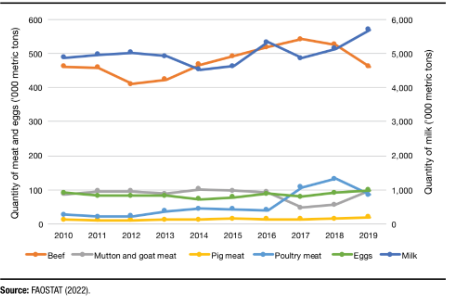
\includegraphics[width=0.9\textwidth]{figures/FAOSTAT_production_trends.png}
    \caption{Trends in selected livestock production in Kenya, 2010--2019.}
    \label{fig:livestock-production-trends}
    \caption*{\textit{Source: FAOSTAT (2022).}}
\end{figure}

Historical trends of livestock production also suggest a close association between changes in output and changes in livestock numbers, but not necessarily in proportional terms. At continental level, the African Union’s Livestock Development Strategy for Africa states that increases in herd and flock size have contributed significantly to the growth in the supply of beef, milk, poultry and sheep and goat meat % TODO: cite (African Union, 2015). This finding suggests that population dynamics should be understood in the future assessment of livestock supply and that the growth of livestock populations may add to total production without being reflected in equivalent productivity increases. 

Evidence from Kenya’s smallholder dairy sector further illustrates the relationship between livestock population structure and production. % TODO: cite Wanjala and Njehia, (2014) noted that poor performance of dairy herd was associated with inadequate replacement stock, limited access to improved breeding animals, inadequate feed quantity and quality, breed characteristics and short lactation periods. The results are dairy cattle specific, but they do suggest a substantial consideration for livestock population and production analysis in general. 

Taken together, the historical evidence suggests that the evolution of livestock populations and the productive characteristics of those populations should both be taken into account in forecasting livestock production. The variation across livestock commodities and the importance of herd structure and replacement dynamics identified in previous studies also imply that forecasts based purely on aggregate historic growth rates may overlook changes that occur within livestock populations over time. A more disaggregated approach can therefore be a basis for studying how changes in livestock numbers translate into production and then into livestock feed requirements. This allows for cohort-based forecasts of livestock population, production and feed demand for Kenya’s livestock value chains.

\subsection{Modelling Approaches for Livestock Population and Production Forecasting}

Different modeling approaches have been used in past studies to project future livestock production and supply. A common approach is extrapolation of historical growth rates in which past trends in production are used to generate probabilistic estimates of future livestock supply. Other studies have used exploratory scenario-based models which start from current production conditions and assess how different drivers, trends and interactions may influence future livestock production  % TODO: cite (Wiebe et al., 2018). 

More sophisticated approaches integrate economic relationships with biophysical factors such as land-system changes, crop physiology and water availability to estimate future agricultural and livestock supply, including integrated assessment and partial-equilibrium models  % TODO: cite (Robinson et al., 2015). Projections have also been developed in Kenya based on assumptions of changes in livestock production over time. 

Statistical modeling approaches have also been used to explore factors that drive livestock productivity in Kenya. For instance,  % TODO: cite Ajak et al. (2020) employed linear regression to assess the relationship between productivity of dairy cattle and factors including concentrate feeding, breed and disease. The analysis found a positive association between milk production and concentrate feeding in early lactation, and reproductive and productive performance was associated with management and production-related factors. The primary aim of such regression-based approaches, however, is explanatory rather than predictive. However regression models can provide an important basis for forecasting by identifying production drivers that may be incorporated as explanatory variables in future livestock production models. 

\subsection{Cohort-Based Herd Dynamics, Population and Production Projection Models}

Cohort-based, age and sex-stratified models divide livestock populations into biologically meaningful groups and simulate movement through successive stages based on reproduction, maturation, mortality and removal rates. An early basis for this approach was the ILCA cattle herd-dynamics model of % TODO: cite Konandreas and Anderson (1982). The model simulated herd development in a stochastic demographic framework for evaluating production alternatives. Later stage-structured approaches, e.g. % TODO: cite  Hary (2004), showed that sustainability of livestock production depends not only on herd size but also on the demographic composition of the herd and on the pattern of animal off-take. 

Empirical applications have highlighted the significance of explicitly considering the population structure of livestock. For example, % TODO: cite  Lesnoff, Corniaux and Hiernaux (2012) used a demographic model to study the recovery of the cattle population after drought and showed that the recovery was particularly sensitive to reproductive performance. Likewise, % TODO: cite  Tuffa and Treydte (2017) developed a stochastic age and sex-structured model for Boran cattle which included demographic processes, carrying capacity, market conditions and herder decisions. Their results suggested that decisions to remove animals from different demographic groups can drastically change population trajectories. Combined, these studies indicate that livestock population projections are more informative when they include the demographic processes by which populations are replenished, mature and removed, rather than just using aggregate growth rates. 

\subsection{Biological Transition Parameters: Mortality, Reproduction, Maturation and Off-take}

Studies from across Sub-Saharan Africa have documented significant differences in mortality, fertility, maturation and off-take rates across livestock species and production environments. In a systematic review of livestock production parameters, % TODO: cite Otte and Chilonda (2002) summarized the relative high mortality of young cattle and small ruminants, low reproductive performance and generally low off-take in traditional production systems. Their synthesis also showed that population growth rates vary widely among species and production systems, emphasizing the necessity of biologically and geographically relevant transition parameters. Off-take is important especially as animals may leave the herd by sale or slaughter before the end of their biological life. These processes imply that the observed changes in livestock population are the net result of births, maturation, mortality and removals. 

\subsection{Production-System Modelling Across Livestock Value Chains}

Population projections need to be converted into production with parameters reflecting the biological and management characteristics of individual livestock value chains. As earlier research in Kenya has shown, there are large variations in productivity between livestock species and production systems. For example, research on smallholder dairy systems has found relatively low milk yields, long calving intervals and large feed-related productivity constraints % TODO: cite (Kashongwe et al., 2017). Studies of genetics have also revealed that patterns of lactation in smallholder systems differ from those under intensive production conditions, adding to the need for production parameters that are indicative of the local production environments % TODO: cite (Ojango et al., 2019). 

A similar differentiation is needed in other value chains. For instance, the Kenyan poultry sector is characterized by distinct indigenous and commercial production systems with very different population dynamics and production characteristics % TODO: cite (Magothe et al., 2012). Population changes are also converted into meat output in beef and small ruminant systems thru species and system specific growth and offtake characteristics. Camel production is a growing component of livestock-based livelihoods in the arid and semi-arid lands. International frameworks such as FAO's GLEAM also connect livestock populations with species-specific production outputs % TODO: cite (FAO, 2018). The studies suggest that a single population to production relationship may not adequately capture the diversity of the Kenyan livestock sector, thereby justifying the use of production parameters that are specific to each value chain. 

\subsection{Carrying Capacity, Feed Availability and Feed Demand}

Availability of feed resources also limits the growth of the livestock population. Studies of carrying capacity in African rangelands show that livestock numbers must be matched against available forage, and remote-sensing studies have increasingly made it possible to include seasonal and spatial variation in forage availability in livestock assessments % TODO: cite (Meshesha et al., 2019). 

Conventional livestock feed balance methods calculate how dry matter animals need by looking at their body weight or using livestock unit equivalents. Common intake rates like the 2.5 percent of body weight per day standard have been helpful for figuring out how much feed animals need when doing livestock assessments % TODO: cite (Rivière, 1991; Kearl, 1982). Applications across Sub-Saharan Africa have used these approaches to identify substantial and often seasonal feed deficits. These developments suggest that livestock population and production projections can provide a useful basis for estimating future feed requirements. 

\subsection{Research Gap}

The reviewed literature establishes each component of the present study on solid empirical and methodological ground: cohort-structured herd models are validated and generalisable % TODO: cite (Konandreas & Anderson, 1982; Hary, 2004; Lesnoff et al., 2012; Tuffa & Treydte, 2017); biological transition parameters for Sub-Saharan systems are documented in synthesis form % TODO: cite (de Leeuw & Wilson, 1988; Otte & Chilonda, 2002); species-specific production has been characterised across Kenya's key value chains % TODO: cite (Magothe et al., 2012; Kashongwe et al., 2017; Ojango et al., 2019); satellite-based forage and carrying-capacity estimation researched % TODO: cite (Meshesha et al., 2019); dry-matter feed-balance methods are standardised % TODO: cite (Rivière, 1991; Kearl, 1982); and integrated scenario frameworks have demonstrated policy relevance for Kenya % TODO: cite (Bosire et al., 2022; FAO, 2018).

What remains scarce is a single, reproducible, biologically grounded framework that unifies these strands for Kenya. One that simultaneously (i) spans all nine key value chains rather than a single species, (ii) advances cohort transitions at a quarterly time step to capture seasonality, (iii) endogenously constrains herd growth through a dynamic feed-supply balance driven by satellite-derived carrying capacity, and (iv) closes the loop from population to species-specific production to disaggregated feed demand. Existing Kenyan analyses are typically either static inventories % TODO: cite (KNBS, 2019), single-value-chain studies, or top-down economic-scenario projections that do not resolve underlying herd demography. By integrating these elements into one coherent, parameter-transparent architecture, the present study addresses a clear and consequential gap, offering not only defensible forecasts but a diagnostic instrument for identifying the feed deficiencies, low off-take rates and reproductive bottlenecks that aggregate assessments obscure.

